\entry{2026-10-20}{Priority 3: test space, quadrature, rule families and a qualified 3D speed-up}

Lane \texttt{2026-10-18-jcp-dims}, last commit \texttt{a99906fe6}, mirror \texttt{038cce675}. H200 jobs (\texttt{jax\_backend=gpu}), 35.2 of 55 GPU-h, nothing deferred; results audit 2 ACCEPT, report audit 5 ACCEPT. Numbers quoted from the generated \path{report.md}; error-based verdicts are E0-conditional.

\begin{itemize}
\item \textbf{A4 (smallest qualifying quadrature, 2D):} 22 of 26 $(r,M)$ cells reach a Gauss $m^\star$ (9{,}216--36{,}864 points); the 4 square cells ($M=r$) reach none.
\item \textbf{A3 (2D factorial):} 128$\to$256$\to$384 improve, 384$\to$512 does not --- the same regression as priorities 1--2.
\item \textbf{B6 (test space):} the deliberately weak $M=r$ control is unavailable --- none of 108 square configurations passes solver qualification. A low mixed-frequency test set is stable but needs 4$\times$ more Gauss points; accuracy inconclusive.
\item \textbf{B3 (rule families):} Fibonacci lattice $m^\star$ 4{,}181--28{,}657 in 2D; Gauss and lattice tie at $m^\star=32{,}768$ in 3D; Halton, Sobol and Monte Carlo are flagged by the cross-family gate; the bad-vector control fired in 2D and 3D.
\item \textbf{2D cost elasticities:} about 0.65 in $r$, 0.53 in $M$, 0.65 in $m$.
\item \textbf{A qualified 3D speed-up:} the 3D quadrature search found qualified configurations at every width (2--32 each). The cheapest that ties or beats each earlier comparator, M2\_512 Gauss $32^3$ QN-BDF2 at $\Delta t=1/60$, is \textbf{2.95$\times$} faster than the qualified W768 setup (pass), 9.87$\times$ faster than the unqualified W1024 setup, and only 1.15$\times$ faster than the old deployment (fails the 1.67$\times$ bar). Coordinator recheck from raw screen timings: 1.19$\times$, 2.98$\times$, 9.75$\times$. This is ROM against ROM; it does not change K2.
\end{itemize}
\begin{center}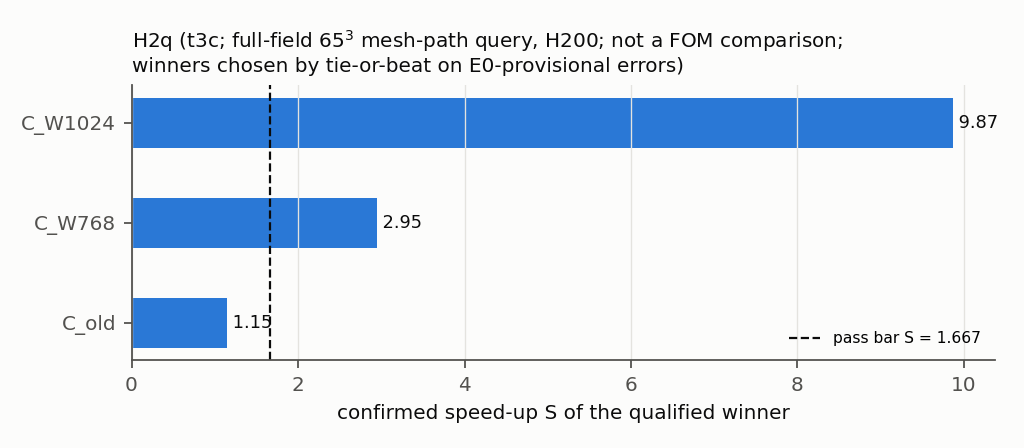
\includegraphics[width=0.48\linewidth]{figs/d_h2q_3d.png}\hfill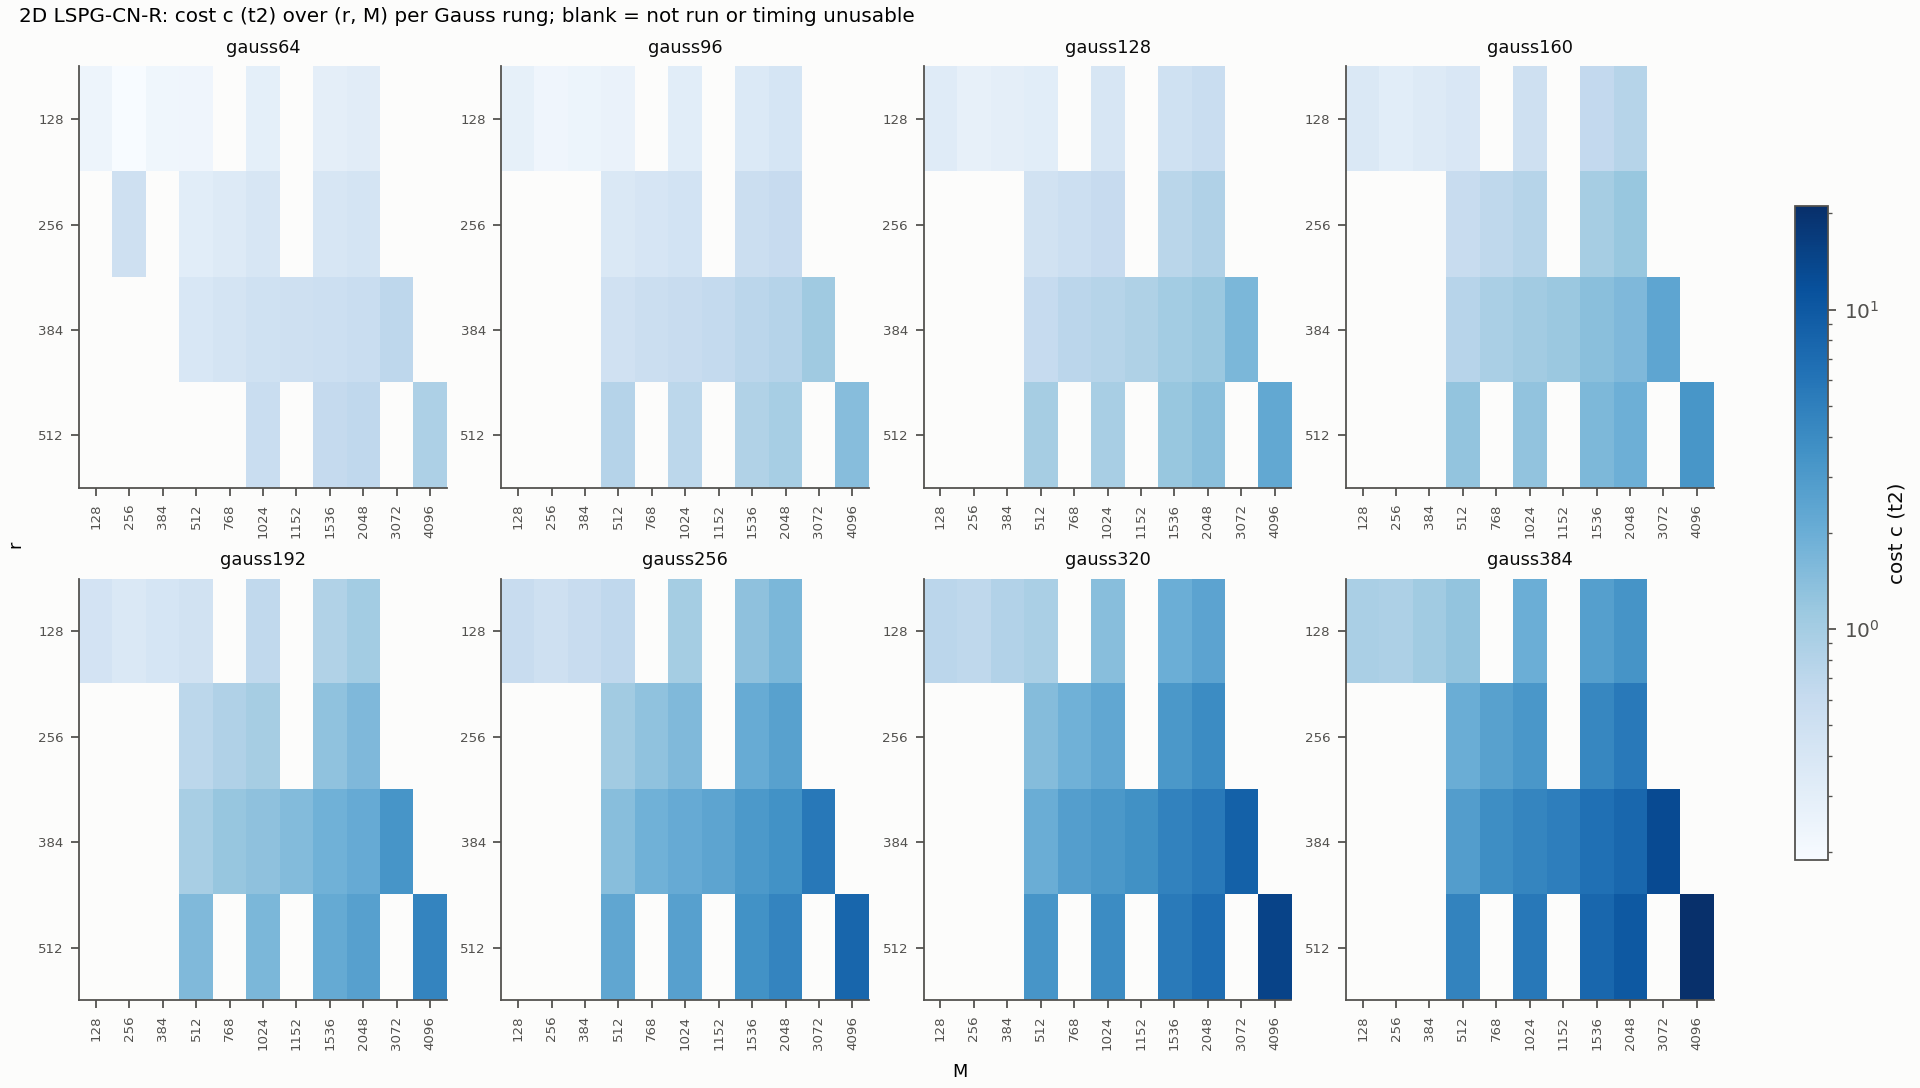
\includegraphics[width=0.48\linewidth]{figs/d_heat_cost_2d.png}\end{center}
\subsection*{Corrections}
\retracted{A post-smoke relaxation of the certificate bar is now stated as such (A6.1/A9.1); the discrepancy figures first given for it were wrong and are replaced. Time estimates for two jobs were too low (reruns, A7, A10.2). The registered timing-identity checks had not been implemented before the first timing config; fixed before submission (A14). One job hit its time limit and its last setting was rerun (A16).}
